%%%%%%%
% Ch3       %
%%%%%%%

\chapter{Convertisseurs à thyristors}
	On s'intéressera aux redresseurs/onduleurs à thyristors ayant une tension de sortie commandable et inversible. Il s'agit de ponts obtenus en remplaçant les diodes par des thyristors. On a aussi les \textbf{ponts mixtes} avec en plus des diodes, mais ne sont pas inversible. On s'attardera aux gradateurs et cycloconvertisseurs qui réalisent une conversion AC/AC sans passer par le DC. Les gradateurs peuvent être constitués de \textbf{triacs}, interrupteur semi-commandable \textbf{bidirectionnel} en courant. 
	
	\section{Caractéristiques des thyristors}
		\begin{wrapfigure}[8]{l}{7cm}
		\vspace{-5mm}
		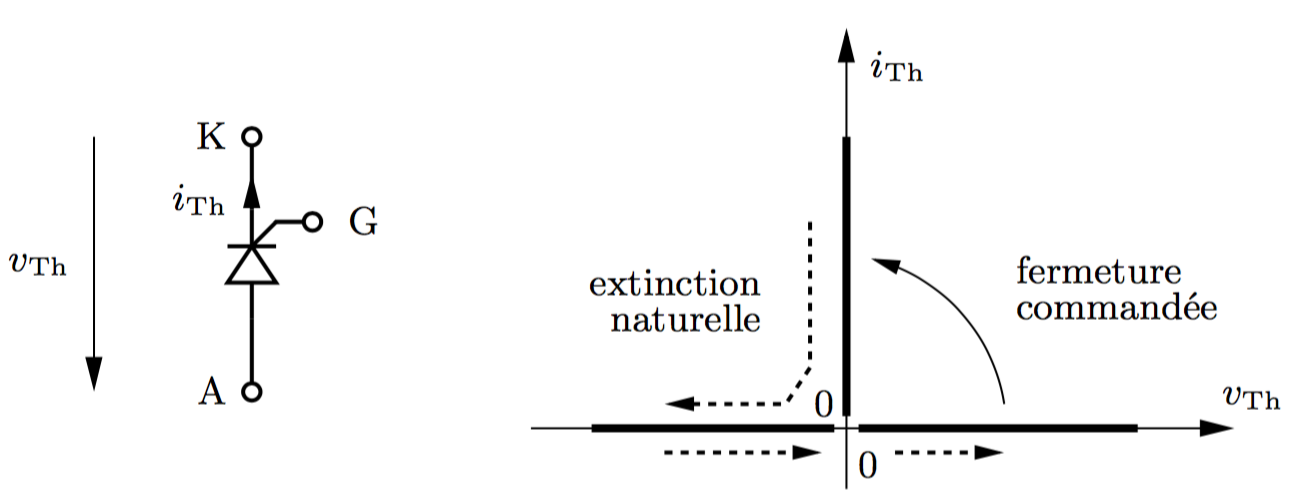
\includegraphics[scale=0.3]{ch3/1}
		\captionof{figure}{} 
		\label{fig:3.1}
		\end{wrapfigure}
		Le thyristor est représenté sur la \autoref{fig:3.1}. En conduction le courant $i_{Th} > 0$ circule de l'anode A vers la cathode K et la \textbf{gâchette G} permet d'amorcer la conduction. Il a le même comportement qu'une diode. Polarisé en \textbf{inverse} $V_{AK}<0$, il y a un courant de fuite $<0$ négligeable. Polarisé en \textbf{direct}, il ne conduira que lors d'impulsion de courant positive dans la gâchette. Comme la diode, le thyristor s'éteint sans qu'une commande ne soit donnée, lorsque le courant s'annule. C'est pourquoi il est \textbf{semi-commandable}. On peut le rendre commandable (sans annulation naturelle du courant), on peut le munir d'un circuit auxiliaire de commutation, mais aux dépens d'une complexité et des pertes plus grandes. \\
		
		Les tensions directe et inverse et le courant de conduction supporté peuvent être de plusieurs \textbf{kilo} volts/ampères. La chute de tension en conduction de l'ordre du volt, modélisé par $V_{Th,on}$ et $R_{Th,on}$. La capacité en fréquence est très limitée. Aucun problème pour la fréquence du réseau, mais pas évident pour une utilisation à plusieurs centaines de hertz. 


	\section{Circuits élémentaires à thyristor}
		\subsection{Circuit avec un thyristor et une charge R}
			Dans ce cas particulier où la source AC est idéale, le courant $i_{ac}(t) = i_{dc}(t)$. Lors des alternances positives, le thyristor est polarisé en direct. L'impulsion dans la gâchette est fournie avec un retard $\alpha$ (rad) appelé \textbf{angle de retard à l'amorçage} compris entre 0 et $\pi$. Quand $v_{ac}$ s'annule et devient négative , $i_{dc}$ et $v_{dc}$ font de même et le thyristor s'éteint naturellement (polarisé en inverse). Voir \autoref{fig:3.2}. On obtient pour la valeur moyenne de la tension redressée :
			\begin{equation}
				V_{dc} = \frac{1}{2\pi}\int _\alpha ^\pi \sqrt{2} V_{ac} \sin \omega t \, \omega t = \frac{\sqrt{2}}{\pi} \frac{1+\cos \alpha}{2} V_{ac}.
			\end{equation}
			
			\begin{minipage}{0.46\textwidth}
				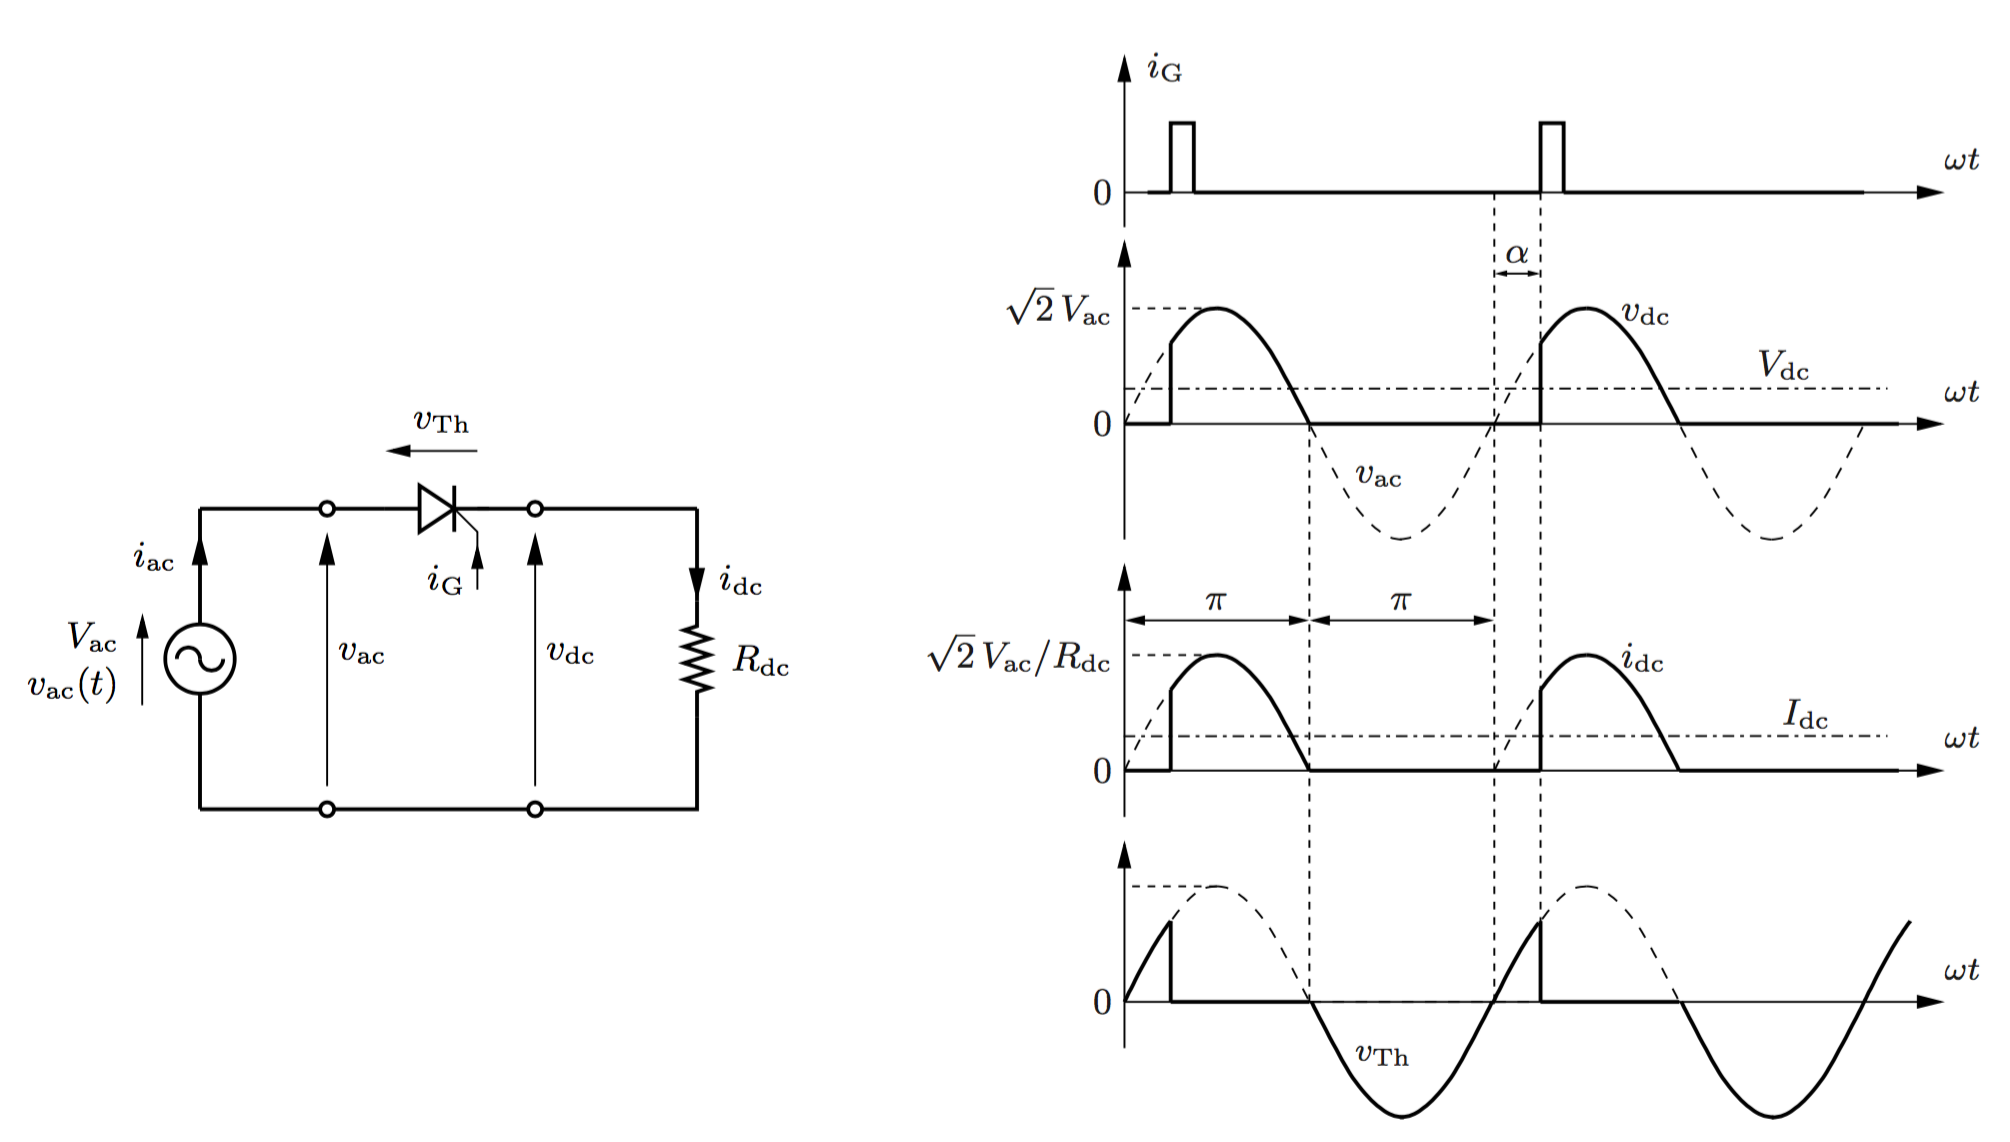
\includegraphics[scale=0.22]{ch3/2}
				\captionof{figure}{}
				\label{fig:3.2}
			\end{minipage}
			\begin{minipage}{0.46\textwidth}
				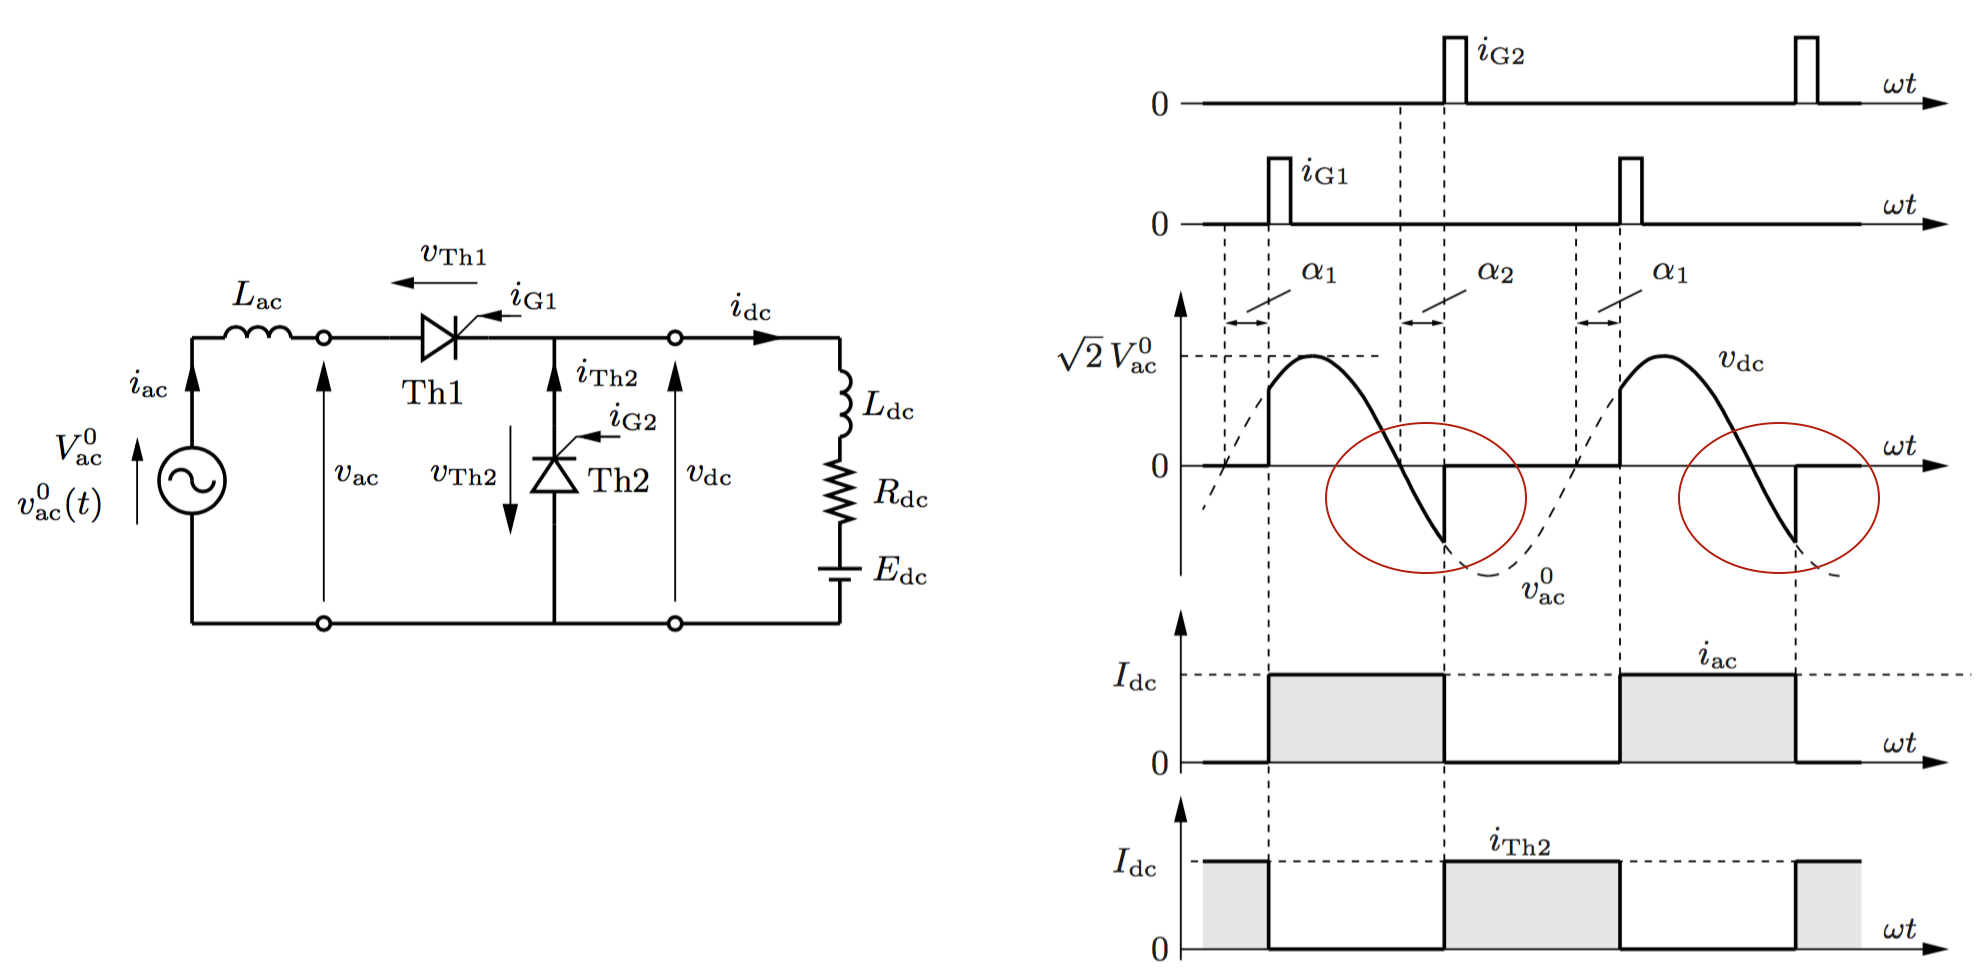
\includegraphics[scale=0.22]{ch3/3}
				\captionof{figure}{}
				\label{fig:3.3}
			\end{minipage}
			
		\subsection{Circuit avec un thyristor redresseur et un thyristor de roue libre}
			Cette configuration est représentée sur la \autoref{fig:3.3}, où on retrouve 2 diodes Th1 et Th2. On discute 2 cas suivant la nature de la source.  
			
			\subsubsection{Avec source de tension idéale (sans inductance)}
				Les formes d'onde pour le cas $L_{ac} = 0, L_{dc} = \infty$ se trouvent à la \autoref{fig:3.3}. On peut remarquer que l'intervalle de conduction de Th1 dépend de 2 angles $\alpha _1$ et $\alpha _2$. Quand le $i_{dc}$ circule dans Th2, $v_{dc} = 0$. On suppose que la commutation se fait instantanément. Remarquons que $v_{dc}$ devient négative jusqu'à l'injection de $i_{G2}$. En effet, les 2 thyristors ne peuvent pas conduire en même temps puisque $v_{ac} = v_{Th1} - v_{Th2}$. On voit bien que si $v_{ac} < 0$ et si Th1 conduit, alors $v_{ac} = -v_{Th2} = v_{dc}$. La tension de sortie moyenne est : 
				\begin{equation}
					V_{dc} = \frac{1}{2\pi} \int _{\alpha _1} ^{\pi + \alpha _2} \sqrt{2} V_{ac}^0\sin \omega t \, d\omega t = \frac{\sqrt{2}}{\pi} \frac{\cos \alpha _1 + \cos \alpha _2}{2} V_{ac}^0.
 				\end{equation}
		
			\subsubsection{Avec source de tension non idéale (avec inductance)}
				\begin{wrapfigure}[12]{l}{6cm}
				\vspace{-5mm}
				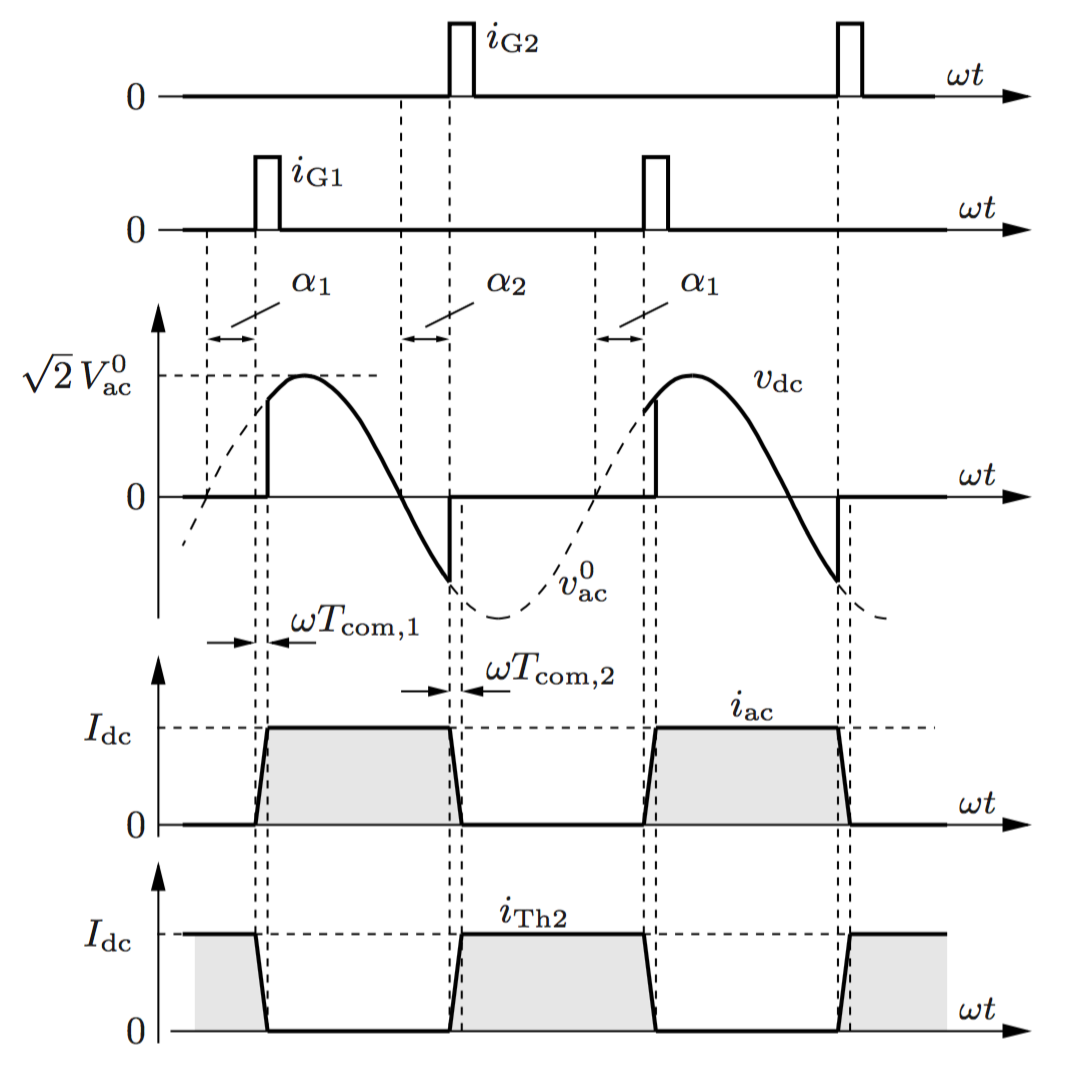
\includegraphics[scale=0.3]{ch3/4}
				\captionof{figure}{} 
				\end{wrapfigure}
				Dans le cas où $L_{ac}$ est non nul, la commutation prend un certain temps. Durant ces intervalles, les thyristors conduisent en même temps et la montée du courant $i_{ac}$ dont le début est contrôlé par $\alpha _1$ et le début de la descente par $\alpha _2$ obéissent à l'équation de la maille de gauche :
				\begin{equation}
					v_{ac}^0 = \sqrt{2} V_{ac}^0 \sin \omega t = L_{ac} \frac{di_{ac}}{dt}. 
				\end{equation}
				La durée de la montée se trouve en intégrant de la sorte :				
				\begin{equation}
				\begin{aligned}
					&\int _{\alpha _1} ^{\alpha _1 + \omega T_{com,1}} \sqrt{2} V_{ac}^0 \sin \omega t \, d\omega t = \int _0^{I_{dc}} \omega L_{ac} \, di_{ac}\\ \Rightarrow\quad &\omega T_{com,1} = \arccos \left( \cos \alpha _1 - \frac{\omega L_{ac}}{\sqrt{2}V_{ac}^0}I_{dc} \right) - \alpha _1
					\end{aligned}
				\end{equation}
				
				Comme on peut le voir, $v_{dc}$ n'est affecté que par les montées. La tension moyenne est donc affectée de la sorte : 
				\begin{equation}
					\Delta V_{dc} = \frac{1}{2\pi} \int _{\alpha _1} ^{\alpha _1 + \omega T_{com,1}} L_{ac} \frac{di_{ac}}{dt} \, d\omega t = \frac{\omega L_{ac}}{2\pi} I_{dc}. 
				\end{equation}
				La tension de sortie moyenne en tenant compte de la chute de tension à travers les thyristors en conduction est :
				\begin{equation}
				V_{dc} = \underbrace{\frac{\sqrt{2}}{\pi} \frac{\cos \alpha _1 + \cos \alpha _2}{2} V_{ac}^0 - V_{Th,on}}_{V_{dc}^0(\alpha _1,\alpha _2)} - \underbrace{\left( R_{Th,on} + \frac{\omega L_{ac}}{2\pi} \right)}_{R_{i,dc}}I_{dc}
				\end{equation}
				Cette équation correspond à un équivalent de Thévenin de la source source de tension DC que constitue la source AC suivie du circuit redresseur. 
				
	\section{Ponts à thyristors monophasé et triphasé}
		\begin{wrapfigure}[11]{l}{10cm}
		\vspace{-5mm}
		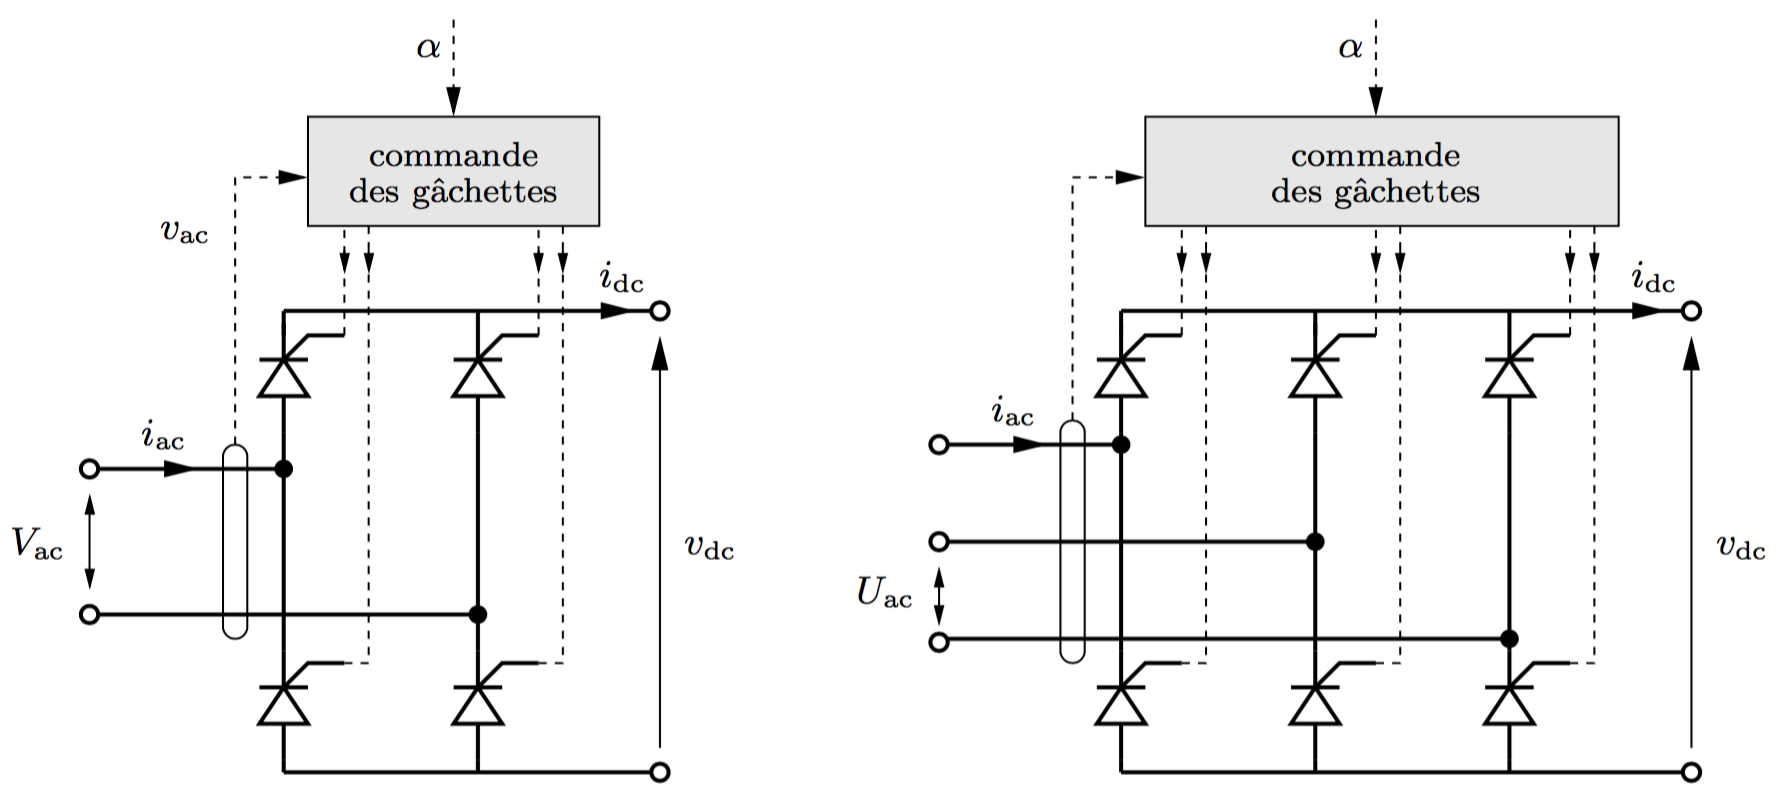
\includegraphics[scale=0.3]{ch3/5}
		\captionof{figure}{} 
		\end{wrapfigure}
		Les montages sont repris sur la figure ci-contre. La commande des thyristors est basée sur la variation de $\alpha$ étant défini comme le délai par rapport au début de conduction dans le redresseur de même topologie, mais avec des diodes ($\alpha = 0$). La déformation des différentes grandeurs AC et DC contiennent les mêmes fréquences et rangs. On considérera une charge suffisamment inductive pour pour que la conduction soit ininterrompue. Selon $\alpha$, on aura un redresseur ou un onduleur. Le fonctionnement en onduleur requiert que la charge DC puisse débiter de la puissance. 
		
			\subsection{Fonctionnement en redresseur}
				\subsubsection{Pont monophasé et charge RLE}
					On suppose une source de tension AC idéale. Il faut que $E_{dc} < V_{dc}$ pour que le courant redressé puisse s'établir. \\
					
					\begin{itemize}
					\item[•] \textbf{Charge infiniment inductive}\\
					Sur la \autoref{fig:3.6} gauche, on peut voir les formes d'ondes pour $\alpha \approx 45\degres$. On peut voir que lorsque $v_{ac}$ passe par 0 pour devenir positif, Th2 et Th3 continuent à conduire du fait de l'inductance élevée et des thyristors en attente d'amorçage. Une fois amorcés, ils reprennent la conduction instantanément et l'autre paire se retrouve polarisée en inverse. $I_{dc}$ parfaitement lisse implique $i_{ac}$ en onde carrée. La composante fondamentale $i_{ac,1}(t)$ est cependant en retard par rapport à $v_{ac}(t)$ de déphasage $\phi _1 = \alpha$. Il y correspond une consommation de puissance réactive proportionnelle à $\sin \alpha$. Par ailleurs, on a $I_{ac,1} = \frac{2\sqrt{2}}{\pi}I_{dc}$. Précisons que c'est grâce à l'inductance très élevée qu'on n'a pas d'annulation de $i_{dc}(t)$ quand $v_{dc}(t)<0$ parfois pour $\alpha \neq 0$. 
					\end{itemize}
					
					\begin{center}
					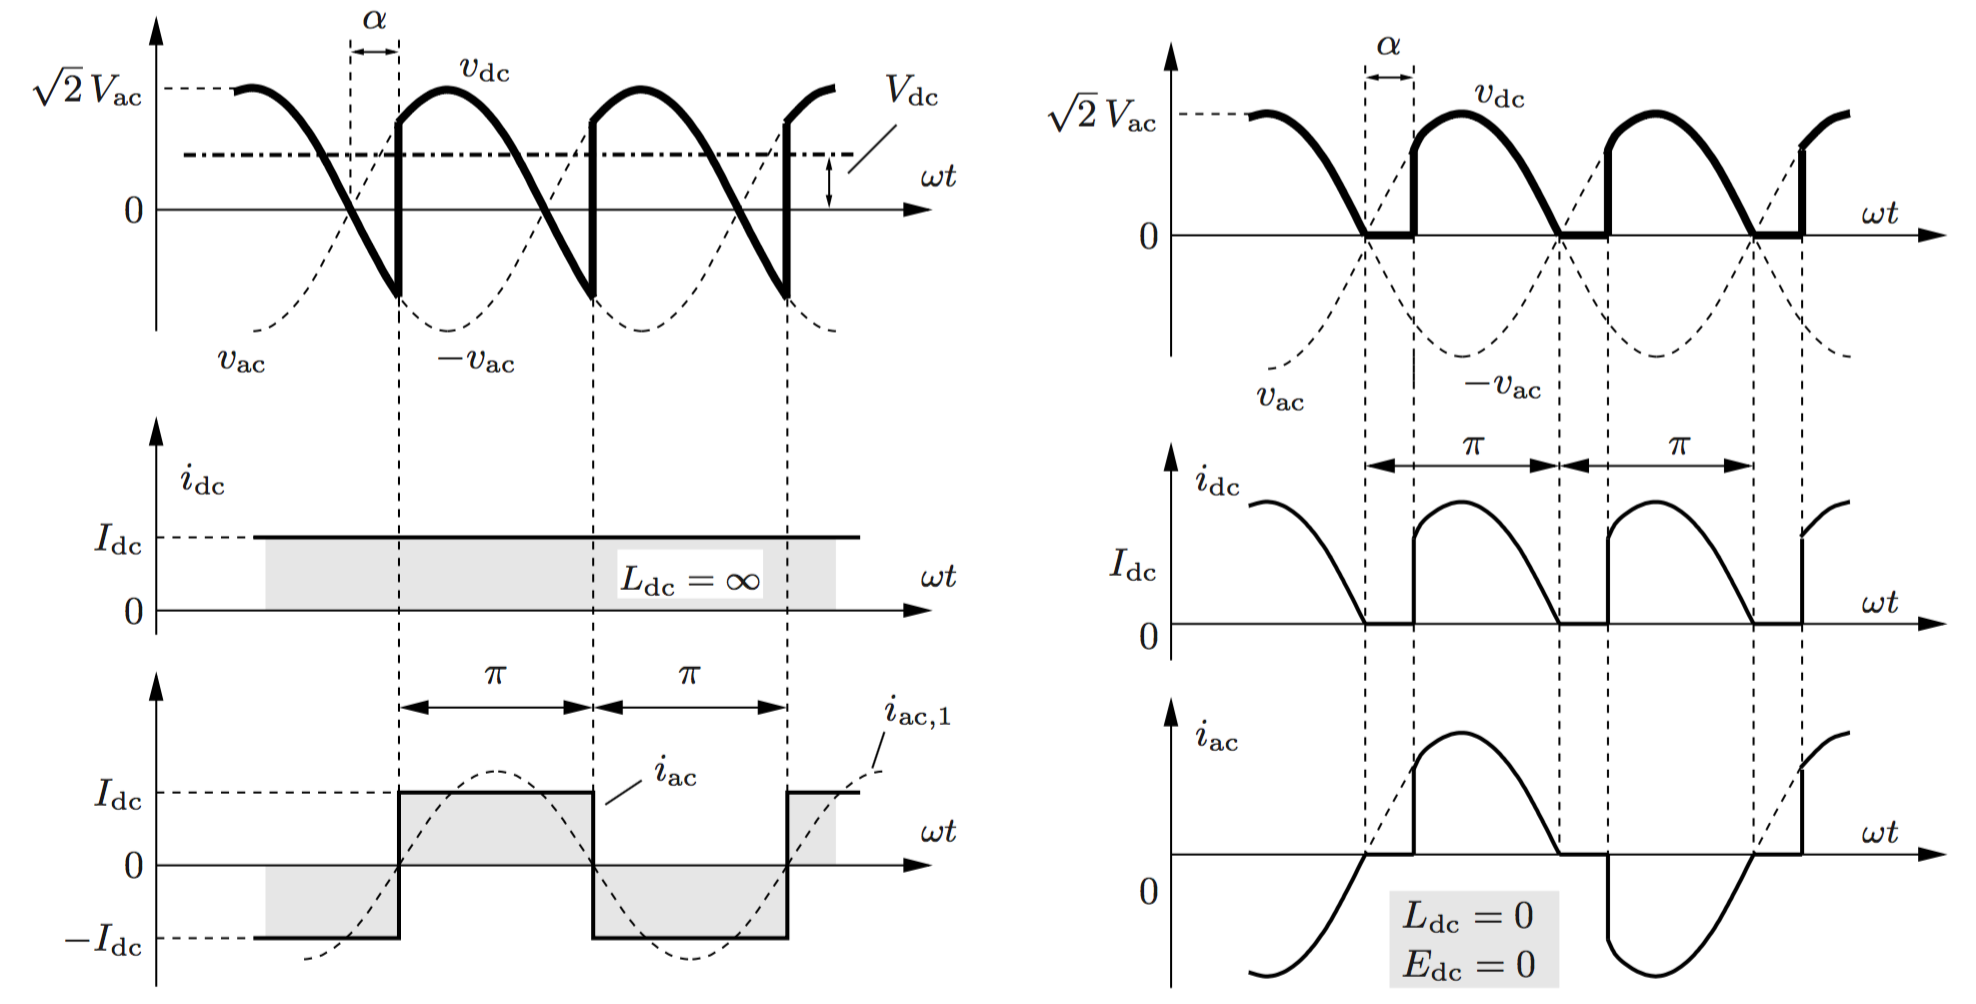
\includegraphics[scale=0.3]{ch3/6}
					\captionof{figure}{}
					\label{fig:3.6}
					\end{center}
					
					\begin{itemize}
					\item[•] \textbf{Charge purement résistive}\\
					Dans ce cas, la conduction est interrompue quelle que soit $\alpha$, puisque ni le courant ni la tension de sortie ne peuvent s'inverser (voir \autoref{fig:3.6} droite). 
					\end{itemize}
					
				\subsubsection{Pont triphasé et charge infiniment inductive}
					\begin{wrapfigure}[12]{l}{5.5cm}
					\vspace{-5mm}
					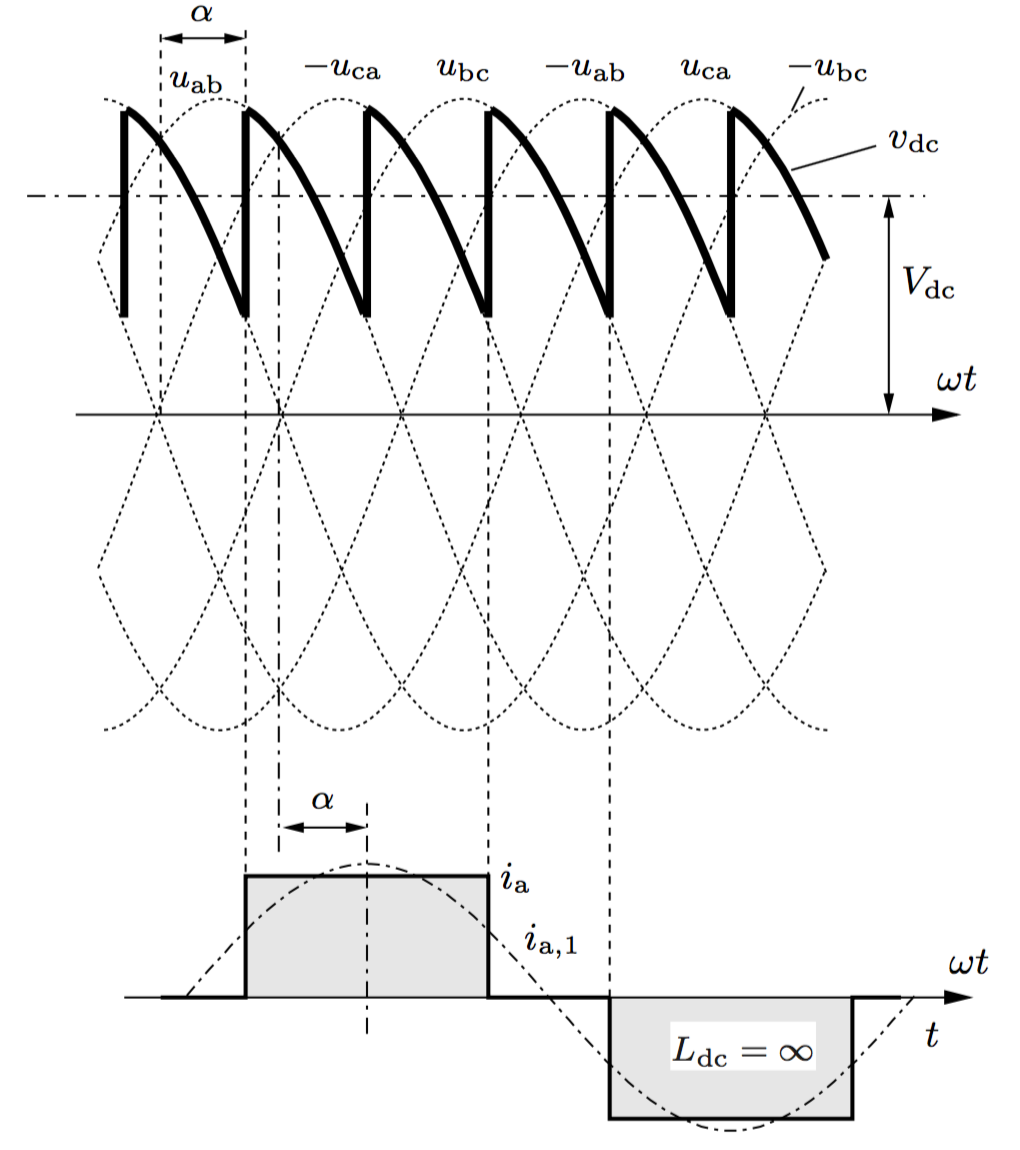
\includegraphics[scale=0.28]{ch3/7}
					\captionof{figure}{} 
					\end{wrapfigure}
					Ci-contre, on trouve les formes d'onde pour $\alpha \approx 40\degres$. Cette fois, l'inductance élevée entraîne $i_{ac}(t)$ en onde carrée triphasée dont $\phi _1 = \alpha$ par rapport à la tension phase-neutre de la phase 1. On a $I_{ac,1} = \frac{\sqrt{6}}{\pi}I_{dc}$. On remarque que la tension de sortie ne devient jamais <0 tant que $\alpha < 60\degres$ et ce dans le cas inductif, car dans le résistif on aurait une conduction interrompue. 
					
				\subsubsection{Tension de sortie moyenne : formules de base (conduction ininterrompue)}
					Pour le cas ininterrompu, il suffit d'ajouter $\alpha$ aux bornes d'intégration pour le même cas avec des diodes :				
					\begin{equation}
					\begin{aligned}
					monophasé &: \frac{1}{\pi} \int _{-\pi /2+\alpha}^{\pi /2 +\alpha} \sqrt{2}V_{ac}\cos\omega t\, d\omega t = \frac{2\sqrt{2}	}{\pi} V_{ac}\cos \alpha \\
					triphasé &: \frac{3}{\pi} \int _{-\pi /6+\alpha}^{\pi /6 +\alpha} \sqrt{2}U_{ac}\cos\omega t\, d\omega t = \frac{2\sqrt{2}	}{\pi} U_{ac}\cos \alpha
					\end{aligned}
					\end{equation}
		
					\begin{wrapfigure}[7]{r}{4.5cm}
					\vspace{-5mm}
					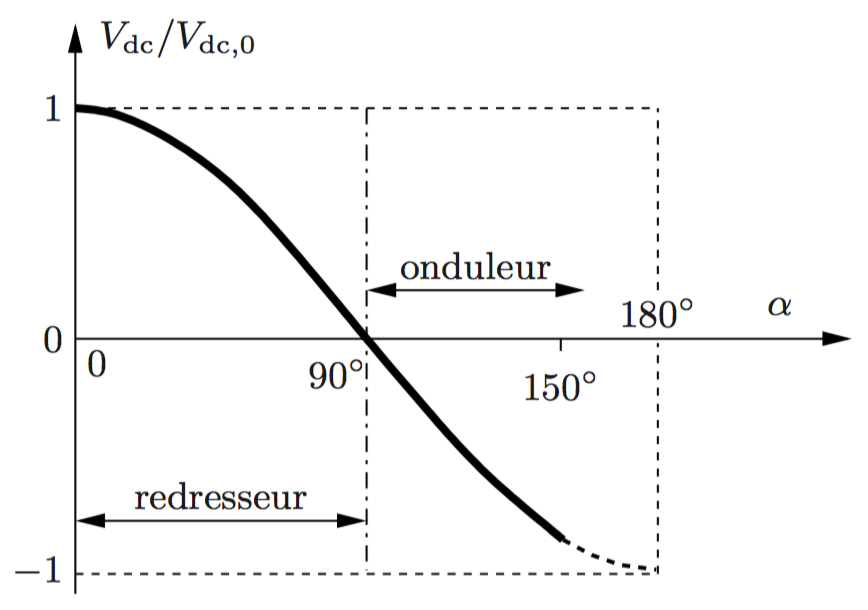
\includegraphics[scale=0.3]{ch3/8}
					\captionof{figure}{} 
					\end{wrapfigure}
					On remarque qu'on aura un maximum en $\alpha = 0$, un zéro en $\alpha = \pi /2$ puis deviendra négative. L'évolution en fonction de $\alpha$ de la tension de sortie moyenne est montrée sur la figure ci-contre. Si maintenant la source possède une inductance et si on prend en compte les chutes de tension des thyristors, on aura des termes en plus et la modélisation en équivalent de Thévenin DC sera possible. 
					
					\newpage
					
			\subsection{Fonctionnement en onduleur (non autonome)}
				\begin{wrapfigure}[13]{l}{5.5cm}
				\vspace{-5mm}
				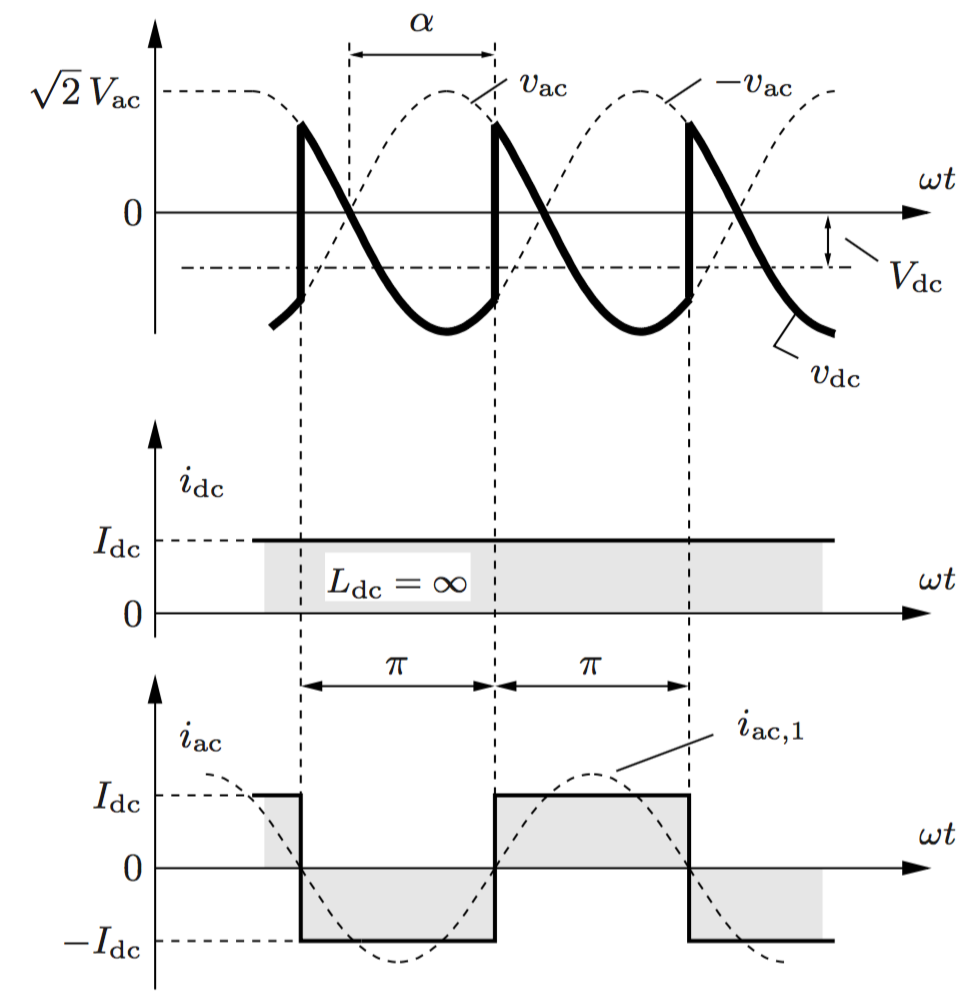
\includegraphics[scale=0.28]{ch3/9}
				\captionof{figure}{} 
				\end{wrapfigure}
				Correspond au cas où $\alpha$ est compris entre 90\degres et 180\degres . La tension moyenne de sortie est négative et la puissance moyenne s'écoule de DC vers AC. On peut voir une représentation des formes d'onde pour $\alpha \approx 135\degres$. Pour rappel, il faut que la charge contienne une source d'énergie comme \textit{l'induit d'une mcc}, on comptera $E_{dc}$ négativement à présent. Comme le courant redressé est positif, il faut en plus que $E_{dc}<V_{dc}$ :
				\begin{equation}
					V_{dc} = E_{dc} + RI_{dc} \qquad \Rightarrow E_{dc} < V_{dc} < 0 
				\end{equation}
				La limite théorique de $\alpha$ est 180\degres ,mais en pratique moins en raison de la durée des commutations. Remarquons par contre qu'on est obligé de raccorder l'entrée à une source de tension AC pour la commande des thyristors, on parle de \textbf{semi-commandabilité} ou encore d'\textbf{onduleurs non autonomes}. Une autre conséquence des thyristors est l'impossibilité de fournir de la puissance réactive au réseau AC. 
				
					\subsubsection{Puissances actives et réactives}
						En considérant une charge ou source DC très inductive et en négligeant la durée de commutation et les pertes dans le pont, pour la \textbf{puissance active} du côté AC on a :
						\begin{equation}
						\begin{aligned}
						monophasé &: V_{ac}I_{ac,1}\cos \alpha = V_{dc}I_{dc}\\
						triphasé &: \sqrt{3}U_{ac}I_{ac,1}\cos \alpha = V_{dc}I_{dc}.
						\end{aligned}
						\end{equation}

						Pour ce qui est de la puissance réactive : 
						\begin{equation}
						\begin{aligned}
						monophasé &: Q_1 = V_{ac}I_{ac,1}\sin \alpha \geq 0\\
						triphasé &: Q_1 = \sqrt{3}U_{ac}I_{ac,1}\cos \alpha \geq 0.
						\end{aligned}
						\end{equation}
						On voit donc qu'on aura toujours de la puissance réactive et qu'elle sera max pour $\alpha = 90\degres$. Inconvénient majeur de ces convertisseurs. La déformation de la tension de sortie est un autre inconvénient. Pour $\alpha = 90\degres$, $v_{dc}$ se présente comme des dents-de-scie à valeur moyenne nulle. 
						
	\section{Ponts mixtes (à diodes et à thyristors)}
		\begin{wrapfigure}[10]{r}{9cm}
		\vspace{-5mm}
		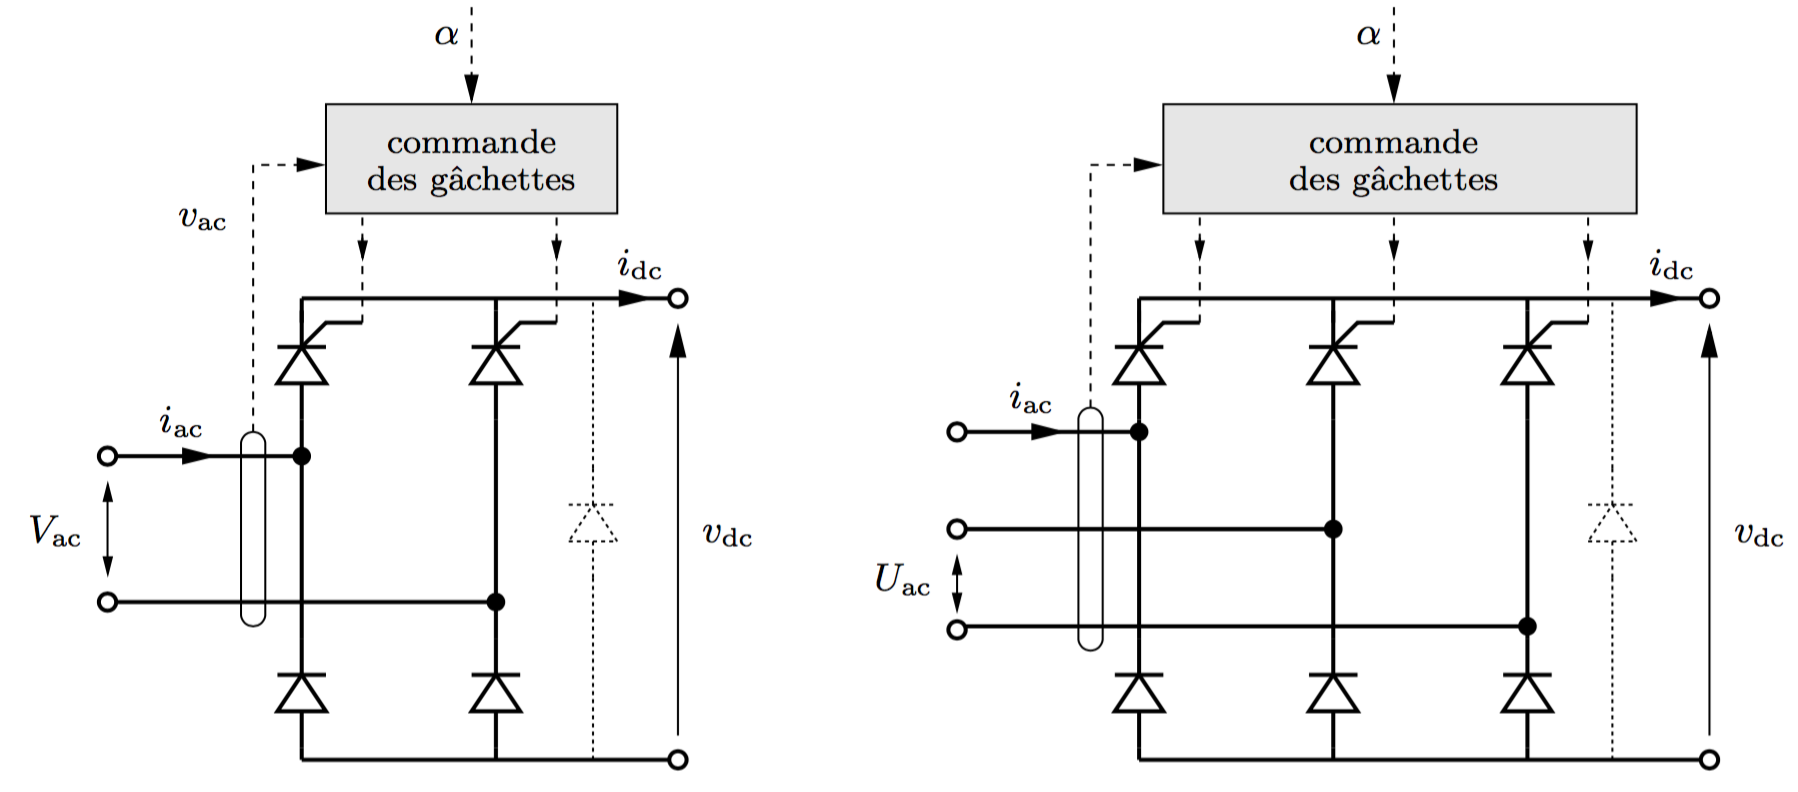
\includegraphics[scale=0.28]{ch3/10}
		\captionof{figure}{} 
		\end{wrapfigure}
		On a des diodes et des thyristors 50/50 (fifty fifty you know) et une diode de roue libre (pointillé) sans réelle influence sur le convertisseur peut être ajoutée. On peut disposer les composants autrement. \\
		
		Regardons d'abord le cas monophasé avec une charge infiniment inductive, une source AC idéale et des composants semi-conducteurs idéaux. Les formes d'onde sont représentées sur la \autoref{fig:3.11}. On peut y voir que $v_{dc}(t)$ ne peut pas être négative. Pour tout $\alpha \neq 0$, il 
		
		\begin{wrapfigure}[10]{l}{5cm}
		\vspace{-5mm}
		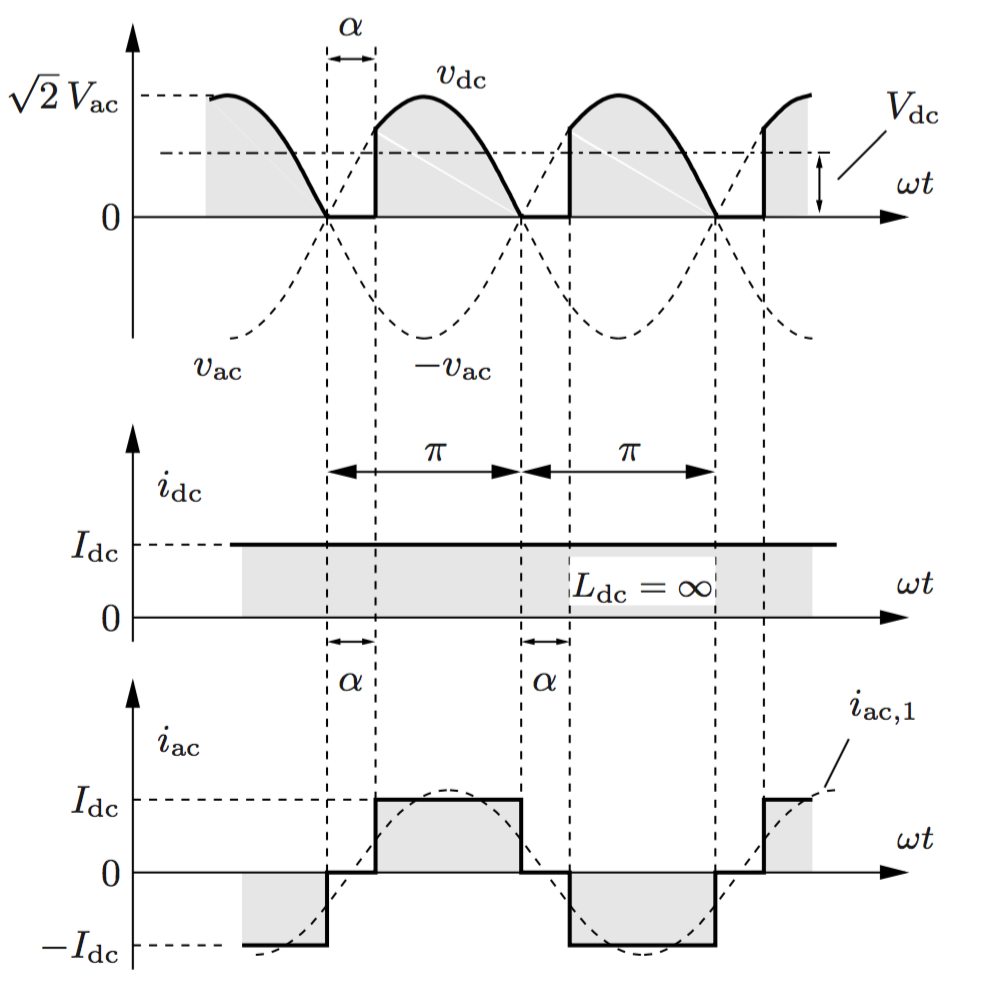
\includegraphics[scale=0.28]{ch3/11}
		\captionof{figure}{} 
		\label{fig:3.11}
		\end{wrapfigure}
		existe donc des intervalles à tension de sortie nulle où la charge DC est court-circuitée à travers l'un des bras ou la diode de roue libre (aucun courant de AC). La tension de sortie moyenne est donnée par : 
		\begin{equation}
			V_{dc} = \frac{1}{\pi} \int _{-\pi /2 +\alpha} ^{\pi /2} \sqrt{2} V_{ac} \cos \omega t \, d\omega t = \frac{2\sqrt{2}}{\pi} V_{ac} \frac{1+\cos \alpha}{2}
		\end{equation}
		c'est à dire la moyenne de la tension de sortie d'un pont tout diode et d'un tout thyristor. La valeur efficace de la composante fondamentale de $i_{ac,1}$ est donnée par : 
		\begin{equation}
			I_{ac,1} = \frac{2\sqrt{2}}{\pi} \cos \frac{\alpha}{2} I_{dc}.
		\end{equation}
		Son angle de retard $\phi _1 = \alpha /2$. Aussi, la déformation du courant AC tend à augmenter avec $\alpha$. On a le bilan de puissance : 
		\begin{equation}
			V_{ac}I_{ac,1}\cos\alpha /2= V_{dc}I_{dc}. 
		\end{equation}
		Comme la tension de sortie est toujours positive en moyenne et en instantanée, ils ne peuvent fonctionner en onduleur. Leur avantage est la complexité et le coût moindre. \\
		
		Pour ce qui est du cas triphasé, on a la sortie moyenne suivante : 
		\begin{equation}
			V_{dc} = \frac{3}{\pi} \int _{-\pi /6 + \alpha}^{\pi /6} \sqrt{2} U_{ac} \cos \omega t \, d\omega t = \frac{3\sqrt{2}}{\pi}U_{ac} \frac{1+\cos \alpha}{2}
		\end{equation}
		qui est également la moyenne des deux types de convertisseurs. 
		
	\section{Caractéristiques des triacs - gradateurs}
		\begin{wrapfigure}[10]{l}{7cm}
		\vspace{-5mm}
		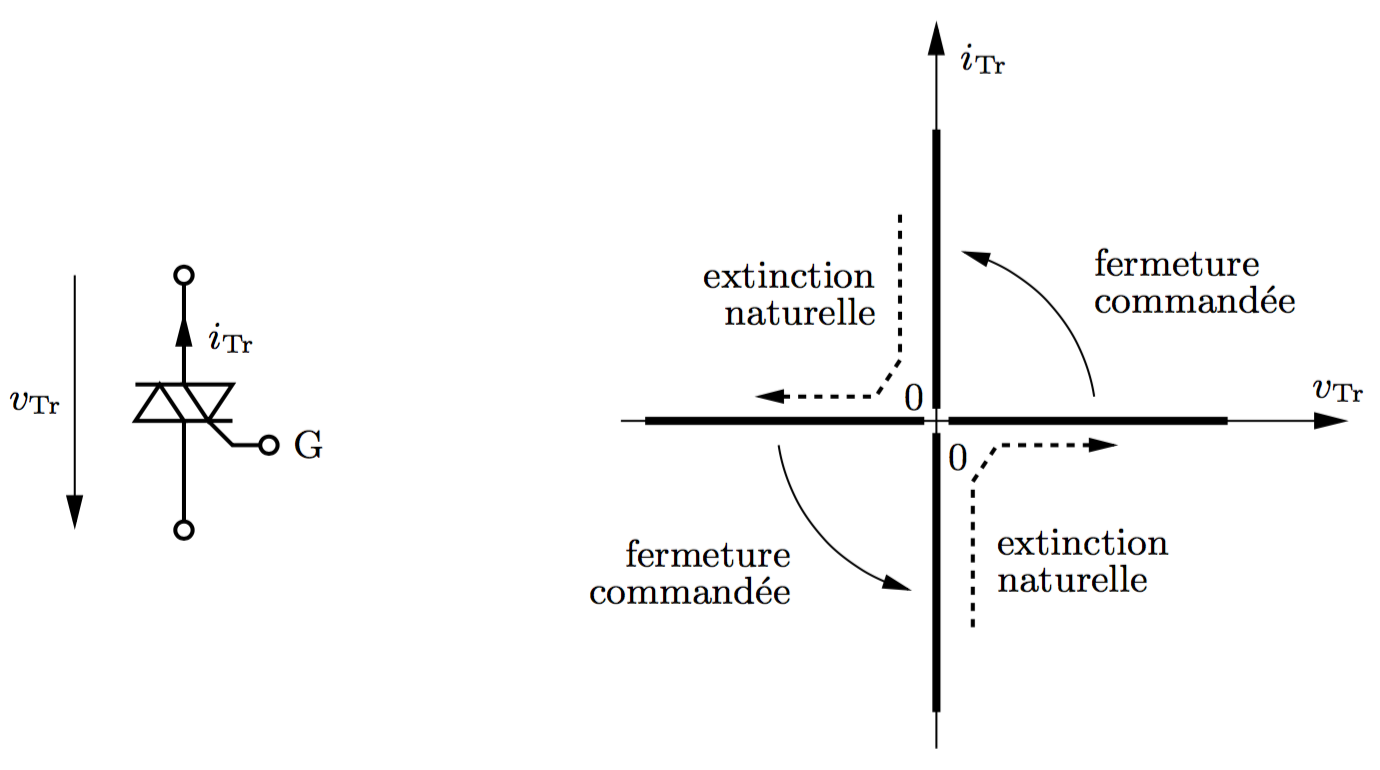
\includegraphics[scale=0.28]{ch3/12}
		\captionof{figure}{} 
		\label{fig:3.12}
		\end{wrapfigure}
		Les gradateurs ou hacheurs à courant AC effectuent une conversion AC-AC, en fréquence inchangée, en monophasé ou en triphasé. Ils sont constitués de triacs ou, pour les grandes puissances, de paires de thyristors montés en tête-bêche. La figure ci-contre montre la bidirectionnalité des triacs en courant. Il se met à conduire dans l'un ou l'autre sens selon le signe de $v_{Tr}$, dès qu'il a reçu une impulsion de courant dans sa gâchette G. De nouveau, annulation naturelle du courant, on ne la commande pas. 
		
			\subsubsection{Gradateurs monophasés}
		 	\begin{wrapfigure}[7]{r}{9cm}
			\vspace{-5mm}
			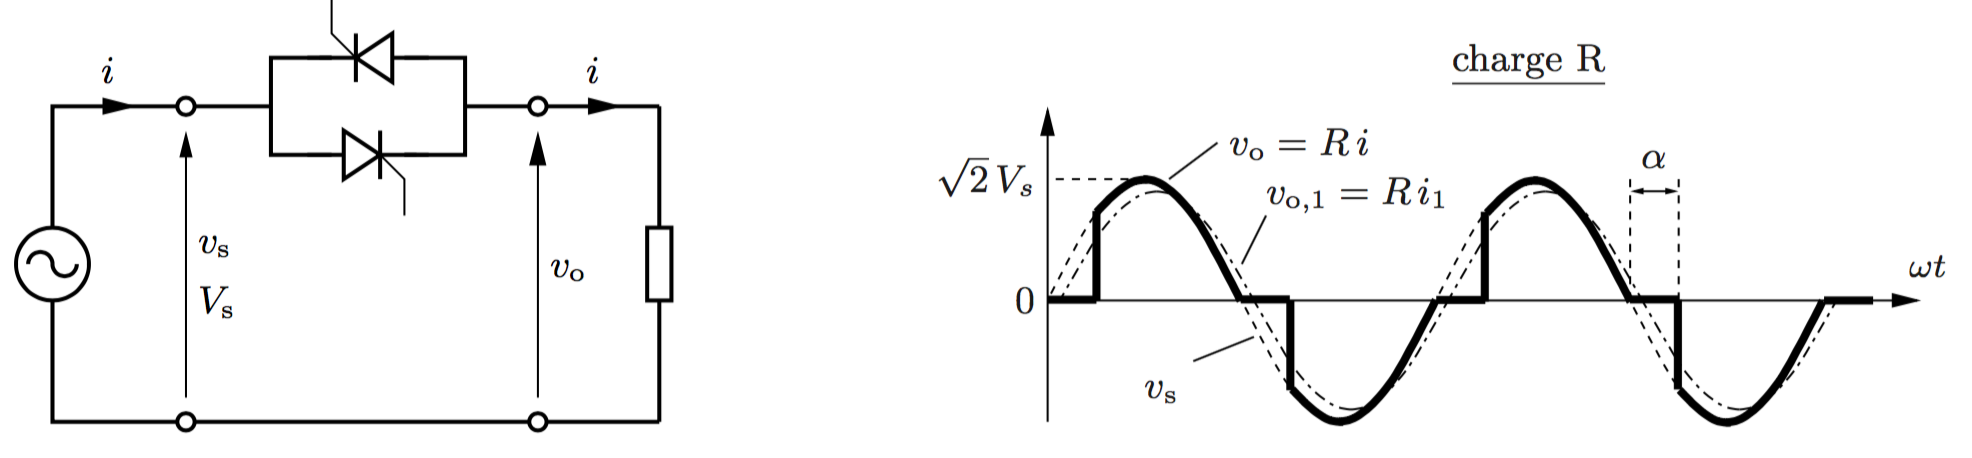
\includegraphics[scale=0.28]{ch3/13}
			\captionof{figure}{} 
			\label{fig:3.13}
			\end{wrapfigure}
			Le circuit comporte 2 thyristors montés en tête-bêche qui équivaut à un triac. La tension de sortie $v_o(t)$ est commandée par l'angle de retard $\alpha$ avec laquelle des impulsions sont envoyées aux thyristors après chaque passage par 0 de la tension d'entrée $v_s(t)$ avec $f_o = f_s$. 
			
			\subsubsection{Charge R}
				Sur la \autoref{fig:3.13} sont montrées les formes d'onde de $v_o(t)$ et $v_{o,1}(t)$ pour le cas d'une charge résistive $v_o(t) = Ri(t)$. Les valeurs efficaces des fondamentaux diminuent et leur retard sur $v_s(t)$ augmente avec $\alpha$. Le gradateur consomme donc de la puissance réactive même lorsqu'il alimente une simple charge R. On a pour la valeur efficace $V_o$ :
				\begin{equation}
					V_o = \sqrt{\frac{1}{\pi}\int _\alpha ^\pi v_s^2 \, d\omega t} = V_s \sqrt{1- \frac{\alpha}{\pi} + \frac{\sin 2\alpha}{2\pi}}. 
				\end{equation}
				Les harmoniques paires sont inexistantes en raison de la symétrie demi-onde et le THD de $v_o$ augmente avec $\alpha$, ce qui est un inconvénient majeur des gradateurs. 
	
	\section{Cycloconvertisseurs}
		\begin{wrapfigure}[12]{r}{8cm}
		\vspace{-5mm}
		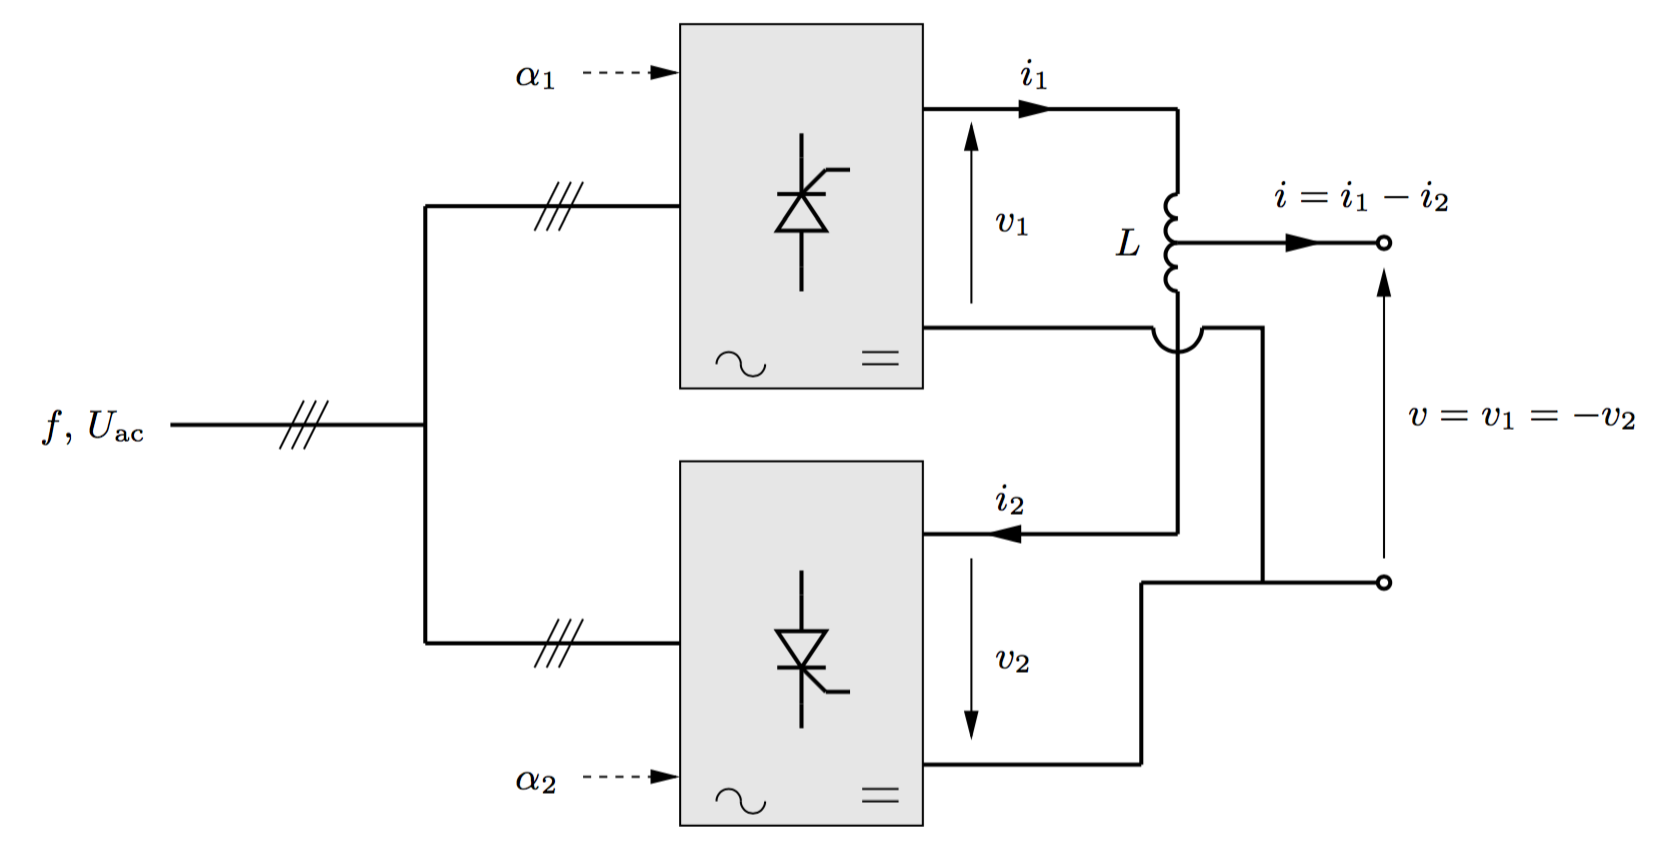
\includegraphics[scale=0.28]{ch3/14}
		\captionof{figure}{} 
		\label{fig:3.14}
		\end{wrapfigure}
		Ce sont des \textbf{convertisseurs de fréquence direct}s, c'est-à-dire qu'il ne passe pas par un bus DC. Ils sont traditionnellement faits de pont à thyristors, mais d'autres topologies existent. Considérons le cycloconvertisseurs à entrée triphasée et sortie monophasée ci-contre, avec 2 ponts à thyristors montés en tête-bêche. Si on fait varier les 2 angles de retard $\alpha _1$ et $\alpha _2$ de façon complémentaire et linéaire dans le temps, donc si $\cos \alpha _1 = - \cos \alpha 2$ et $\frac{d|\alpha _1|}{dt} = \frac{d|\alpha _2|}{dt} = \omega _1$, on obtient une tension de sortie moyenne de : 
		\begin{equation}
			v(t) = 1.35 U_{ac} \cos \alpha _1 (t) = 1.35 U_{ac} \cos (\omega _1 t + \gamma). 
		\end{equation}
		Du fait de $v_1(t) \neq v_2(t)$, un courant de parasite apparaît. On peut le limiter à l'aide d'une inductance par ex. En sélectionnant des morceaux des six tensions phase-phase à l'entrée, on construit notre tension sinusoïdale. Pour que la déformation ne soit pas trop importante, la fréquence de sortie $f_1$ doit être limitée au tiers ou à 40\% de la fréquence d'alimentation. Voir la figure ci-bas. 
		
		\begin{center}
			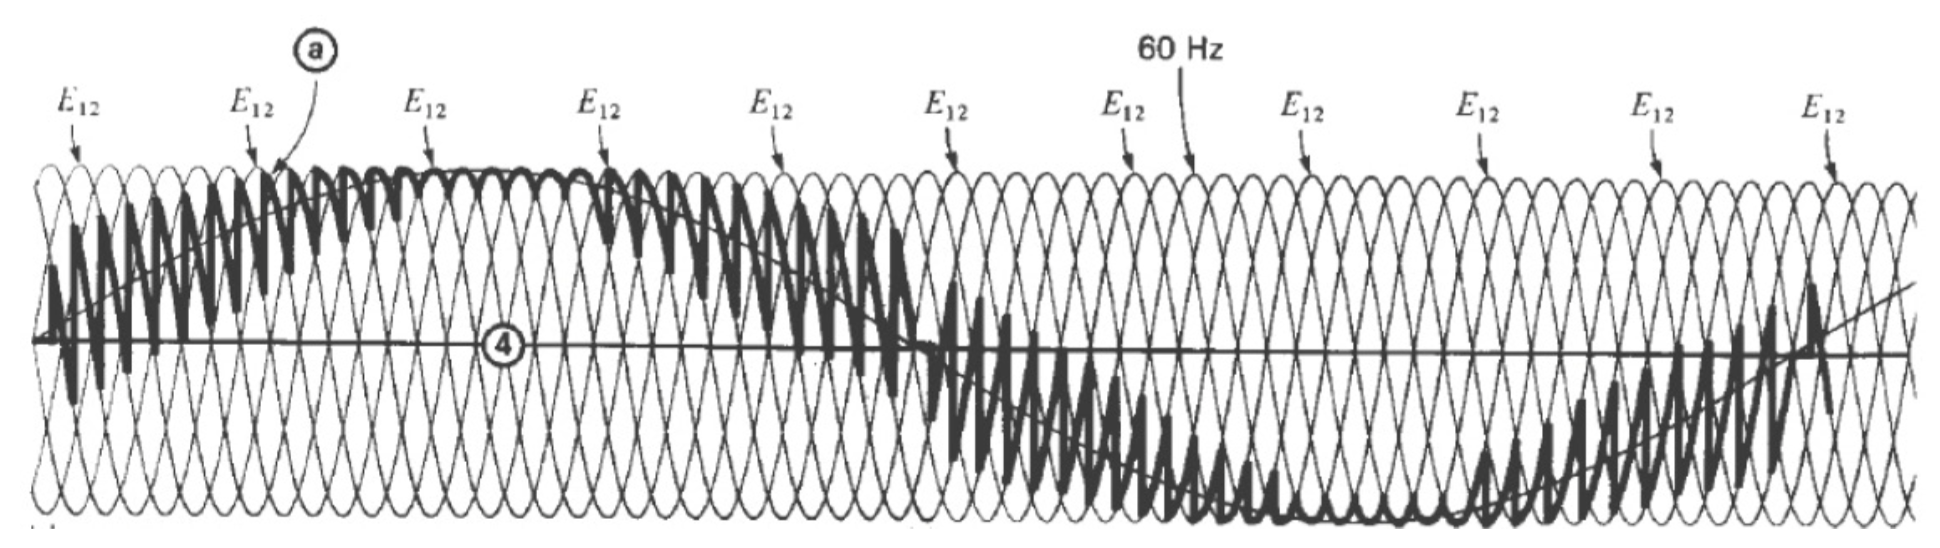
\includegraphics[scale=0.3]{ch3/15}
			\captionof{figure}{}
		\end{center}
